\documentclass[journal,12pt,twocolumn]{IEEEtran}
\usepackage{setspace}
\usepackage{gensymb}
\usepackage{caption}
%\usepackage{multirow}
%\usepackage{multicolumn}
%\usepackage{subcaption}
%\doublespacing
\singlespacing
\usepackage{csvsimple}
\usepackage{amsmath}
\usepackage{multicol}
%\usepackage{enumerate}
\usepackage{amssymb}
%\usepackage{graphicx}
\usepackage{newfloat}
%\usepackage{syntax}
\usepackage{listings}
\usepackage{iithtlc}
\usepackage{color}
\usepackage{tikz}
\usetikzlibrary{shapes,arrows}



%\usepackage{graphicx}
%\usepackage{amssymb}
%\usepackage{relsize}
%\usepackage[cmex10]{amsmath}
%\usepackage{mathtools}
%\usepackage{amsthm}
%\interdisplaylinepenalty=2500
%\savesymbol{iint}
%\usepackage{txfonts}
%\restoresymbol{TXF}{iint}
%\usepackage{wasysym}
\usepackage{amsthm}
\usepackage{mathrsfs}
\usepackage{txfonts}
\usepackage{stfloats}
\usepackage{cite}
\usepackage{cases}
\usepackage{mathtools}
\usepackage{caption}
\usepackage{enumerate}	
\usepackage{enumitem}
\usepackage{amsmath}
%\usepackage{xtab}
\usepackage{longtable}
\usepackage{multirow}
%\usepackage{algorithm}
%\usepackage{algpseudocode}
\usepackage{enumitem}
\usepackage{mathtools}
\usepackage{hyperref}
%\usepackage[framemethod=tikz]{mdframed}
\usepackage{listings}
    %\usepackage[latin1]{inputenc}                                 %%
    \usepackage{color}                                            %%
    \usepackage{array}                                            %%
    \usepackage{longtable}                                        %%
    \usepackage{calc}                                             %%
    \usepackage{multirow}                                         %%
    \usepackage{hhline}                                           %%
    \usepackage{ifthen}                                           %%
  %optionally (for landscape tables embedded in another document): %%
    \usepackage{lscape}     


\usepackage{url}
\def\UrlBreaks{\do\/\do-}


%\usepackage{stmaryrd}


%\usepackage{wasysym}
%\newcounter{MYtempeqncnt}
\DeclareMathOperator*{\Res}{Res}
%\renewcommand{\baselinestretch}{2}
\renewcommand\thesection{\arabic{section}}
\renewcommand\thesubsection{\thesection.\arabic{subsection}}
\renewcommand\thesubsubsection{\thesubsection.\arabic{subsubsection}}

\renewcommand\thesectiondis{\arabic{section}}
\renewcommand\thesubsectiondis{\thesectiondis.\arabic{subsection}}
\renewcommand\thesubsubsectiondis{\thesubsectiondis.\arabic{subsubsection}}

% correct bad hyphenation here
\hyphenation{op-tical net-works semi-conduc-tor}

%\lstset{
%language=C,
%frame=single, 
%breaklines=true
%}

%\lstset{
	%%basicstyle=\small\ttfamily\bfseries,
	%%numberstyle=\small\ttfamily,
	%language=Octave,
	%backgroundcolor=\color{white},
	%%frame=single,
	%%keywordstyle=\bfseries,
	%%breaklines=true,
	%%showstringspaces=false,
	%%xleftmargin=-10mm,
	%%aboveskip=-1mm,
	%%belowskip=0mm
%}

%\surroundwithmdframed[width=\columnwidth]{lstlisting}
\def\inputGnumericTable{}                                 %%
\lstset{
%language=C,
frame=single, 
breaklines=true,
columns=fullflexible
}
 

\begin{document}
%
\tikzstyle{block} = [rectangle, draw,
    text width=3em, text centered, minimum height=3em]
\tikzstyle{sum} = [draw, circle, node distance=3cm]
\tikzstyle{input} = [coordinate]
\tikzstyle{output} = [coordinate]
\tikzstyle{pinstyle} = [pin edge={to-,thin,black}]

\theoremstyle{definition}
\newtheorem{theorem}{Theorem}[section]
\newtheorem{problem}{Problem}
\newtheorem{proposition}{Proposition}[section]
\newtheorem{lemma}{Lemma}[section]
\newtheorem{corollary}[theorem]{Corollary}
\newtheorem{example}{Example}[section]
\newtheorem{definition}{Definition}[section]
%\newtheorem{algorithm}{Algorithm}[section]
%\newtheorem{cor}{Corollary}
\newcommand{\BEQA}{\begin{eqnarray}}
\newcommand{\EEQA}{\end{eqnarray}}
\newcommand{\define}{\stackrel{\triangle}{=}}

\bibliographystyle{IEEEtran}
%\bibliographystyle{ieeetr}

\providecommand{\nCr}[2]{\,^{#1}C_{#2}} % nCr
\providecommand{\nPr}[2]{\,^{#1}P_{#2}} % nPr
\providecommand{\mbf}{\mathbf}
\providecommand{\pr}[1]{\ensuremath{\Pr\left(#1\right)}}
\providecommand{\qfunc}[1]{\ensuremath{Q\left(#1\right)}}
\providecommand{\sbrak}[1]{\ensuremath{{}\left[#1\right]}}
\providecommand{\lsbrak}[1]{\ensuremath{{}\left[#1\right.}}
\providecommand{\rsbrak}[1]{\ensuremath{{}\left.#1\right]}}
\providecommand{\brak}[1]{\ensuremath{\left(#1\right)}}
\providecommand{\lbrak}[1]{\ensuremath{\left(#1\right.}}
\providecommand{\rbrak}[1]{\ensuremath{\left.#1\right)}}
\providecommand{\cbrak}[1]{\ensuremath{\left\{#1\right\}}}
\providecommand{\lcbrak}[1]{\ensuremath{\left\{#1\right.}}
\providecommand{\rcbrak}[1]{\ensuremath{\left.#1\right\}}}
\theoremstyle{remark}
\newtheorem{rem}{Remark}
\newcommand{\sgn}{\mathop{\mathrm{sgn}}}
\providecommand{\abs}[1]{\left\vert#1\right\vert}
\providecommand{\res}[1]{\Res\displaylimits_{#1}} 
\providecommand{\norm}[1]{\lVert#1\rVert}
\providecommand{\mtx}[1]{\mathbf{#1}}
\providecommand{\mean}[1]{E\left[ #1 \right]}
\providecommand{\fourier}{\overset{\mathcal{F}}{ \rightleftharpoons}}
%\providecommand{\hilbert}{\overset{\mathcal{H}}{ \rightleftharpoons}}
\providecommand{\system}{\overset{\mathcal{H}}{ \longleftrightarrow}}
	%\newcommand{\solution}[2]{\textbf{Solution:}{#1}}
\newcommand{\solution}{\noindent \textbf{Solution: }}
\newcommand{\myvec}[1]{\ensuremath{\begin{pmatrix}#1\end{pmatrix}}}
\providecommand{\dec}[2]{\ensuremath{\overset{#1}{\underset{#2}{\gtrless}}}}
\DeclarePairedDelimiter{\ceil}{\lceil}{\rceil}
%\numberwithin{equation}{subsection}
\numberwithin{equation}{section}
%\numberwithin{problem}{subsection}
%\numberwithin{definition}{subsection}
\makeatletter
\@addtoreset{figure}{section}
\makeatother

\let\StandardTheFigure\thefigure
%\renewcommand{\thefigure}{\theproblem.\arabic{figure}}
\renewcommand{\thefigure}{\thesection}


%\numberwithin{figure}{subsection}

%\numberwithin{equation}{subsection}
%\numberwithin{equation}{section}
%\numberwithin{equation}{problem}
%\numberwithin{problem}{subsection}
\numberwithin{problem}{section}
%%\numberwithin{definition}{subsection}
%\makeatletter
%\@addtoreset{figure}{problem}
%\makeatother
\makeatletter
\@addtoreset{table}{section}
\makeatother

\let\StandardTheFigure\thefigure
\let\StandardTheTable\thetable
\let\vec\mathbf
%%\renewcommand{\thefigure}{\theproblem.\arabic{figure}}
%\renewcommand{\thefigure}{\theproblem}

%%\numberwithin{figure}{section}

%%\numberwithin{figure}{subsection}



\def\putbox#1#2#3{\makebox[0in][l]{\makebox[#1][l]{}\raisebox{\baselineskip}[0in][0in]{\raisebox{#2}[0in][0in]{#3}}}}
     \def\rightbox#1{\makebox[0in][r]{#1}}
     \def\centbox#1{\makebox[0in]{#1}}
     \def\topbox#1{\raisebox{-\baselineskip}[0in][0in]{#1}}
     \def\midbox#1{\raisebox{-0.5\baselineskip}[0in][0in]{#1}}

\vspace{3cm}

\title{ 
	\logo{
Linear Algebra through Coordinate Geometry 
	}
}

\author{ G V V Sharma$^{*}$% <-this % stops a space
	\thanks{*The author is with the Department
		of Electrical Engineering, Indian Institute of Technology, Hyderabad
		502285 India e-mail:  gadepall@iith.ac.in. All content in this manual is released under GNU GPL.  Free and open source.}
	
}	

\maketitle

\tableofcontents

\bigskip

\renewcommand{\thefigure}{\theenumi}
\renewcommand{\thetable}{\theenumi}


\begin{abstract}
	
This manual introduces linear algebra through coordinate geometry using a problem solving approach.
\end{abstract}
\section{The Straight Line}
\begin{enumerate}[label=\thesection.\arabic*
,ref=\thesection.\theenumi]
\item The equation of the line between two points $\vec{A}$ and $\vec{B}$ is given by
\begin{equation}
\vec{x} = \vec{A} + \lambda \brak{\vec{A}-\vec{B}}
\end{equation}
%
Alternatively, it can be expressed as
\begin{equation}
\label{eq:line_normal}
\vec{n}^T\brak{\vec{x}-\vec{A}} = 0
\end{equation}
%
where $\vec{n}$ is the solution of
\begin{equation}
\label{eq:normal_slope}
\brak{\vec{A}-\vec{B}}^T\vec{n} = 0
\end{equation}
\item In $\triangle ABC$,
\begin{equation}
\label{eq:linea}
\vec{A}=\myvec{1\\2}
\end{equation}
%
and the equations of the medians through $\vec{B}$ and $\vec{C}$
are respectively
\begin{align}
\label{eq:line_medb}
\myvec{1 & 1}\vec{x}&=5
\\
\myvec{1 & 0}\vec{x}&=4
\label{eq:line_medc}
\end{align}
%
Find the area of $\triangle ABC$.
\\
\solution The centroid $\vec{O}$ is the solution of \eqref{eq:line_medb},\eqref{eq:line_medc} and is obtained 
as the solution
of the matrix equation
\begin{align}
\myvec{1 & 1 \\1 & 0}\vec{x}&=\myvec{5 \\ 4}
\label{eq:line_matrix}
\end{align}
%
which can be solved using the augmented matrix as follows.
\begin{align}
\myvec{1 & 1 & 5\\1 & 0 & 4} \leftrightarrow \myvec{1 & 1 & 5\\0 & 1 & 1}\leftrightarrow  \myvec{1 & 0 & 4\\0 & 
1 & 1}
\end{align}
Thus,
\begin{equation}
\label{eq:lineo}
\vec{O}=\myvec{4\\1}
\end{equation}
% 
Let  $AD$ be the median through $\vec{A}$. Then,
\begin{align}
\frac{\vec{A}+\vec{B}+\vec{C}}{3}&= \vec{O}
\\
\implies \vec{B}+\vec{C}= 3\vec{O}-\vec{A} &= \myvec{11 \\ 1}
\label{eq:line_b+c}
\\
\implies \myvec{1 & 1}\vec{B}+\myvec{1 & 1}\vec{C}&=  \myvec{1 & 1}\myvec{11 \\ 1}
\label{eq:line_ctemp}
\end{align}
%
From \eqref{eq:line_medc} and \eqref{eq:line_ctemp},
\begin{align}
 \myvec{1 & 1}\vec{B} &= 5 
\\
\implies 5+\myvec{1 & 1}\vec{C}&=  12
\\
\implies \myvec{1 & 1}\vec{C}&=  7
\label{eq:line_ctemp2}
\end{align}
From \eqref{eq:line_ctemp2} and \eqref{eq:line_medc}, $\vec{C}$ can be obtained by solving 
\begin{align}
\myvec{1 & 1 \\1 & 0}\vec{C}&=\myvec{7 \\ 4}
\label{eq:line_cmatrix}
\end{align}
using the augmented matrix as
\begin{align}
\myvec{1 & 1 & 7\\1 & 0 & 4} &\leftrightarrow \myvec{1 & 1 & 7\\0 & 1 & 3}\leftrightarrow \myvec{1 & 0 & 4\\0 & 
1 & 3}
\\
\implies \vec{C}&=\myvec{4\\3}
\end{align}
%
From \eqref{eq:line_b+c},
\begin{align}
\vec{B}&=\myvec{11\\1}-\myvec{4\\3}
=\myvec{7\\-2}
\end{align}
%
Thus,
\begin{align}
\frac{1}{2}
\begin{vmatrix}
\vec{A} & \vec{B} &\vec{C}
\\
1 & 1 & 1
\end{vmatrix}
=
\frac{1}{2}
\begin{vmatrix}
1 & 7 & 4\\2 & -2 & 3 \\ 1 & 1 & 1
\end{vmatrix} = 9
\end{align}
\item Summarize all the above computations through a Python script and plot $\triangle ABC$.
\\
\solution
\begin{lstlisting}
https://github.com/gadepall/school/raw/master/linalg/2D/manual/codes/1.2.py
\end{lstlisting}
\end{enumerate}
\section{Orthogonality}
\begin{enumerate}[label=\thesection.\arabic*
,ref=\thesection.\theenumi]
\item $\vec{u}^T\vec{x} = 0 \implies \vec{u} \perp \vec{x}$. Show that 
\begin{align}
\label{eq:orth_parallel}
\vec{u}^T\vec{x}  = \vec{P}^T\vec{x} = 0 \implies \vec{P} =\alpha 
\vec{u}
\end{align}
%
\item The foot of the perpendicular drawn from the origin on the line 
\begin{align}
\label{eq:orth_line}
AB: \vec{u}^T\vec{x}  =\lambda
\end{align}
where
\begin{align}
\vec{u}=\myvec{3 \\ 1}
\end{align}
is $\vec{P}$.  The line meets the $x$-axis at $\vec{A}$ and $y$-axis at $\vec{B}$. Show that $\vec{P} =\alpha 
\vec{u}$ and find $\alpha$.
\\
\solution From \eqref{eq:orth_line},
\begin{align}
\vec{u}^T\vec{A}=\vec{u}^T\vec{B}=\lambda
\\
\implies \vec{u}^T\brak{\vec{A}-\vec{B}}=0
\end{align}
%
Since $OP \perp AB$,
\begin{align}
\vec{P}^T\brak{\vec{A}-\vec{B}}=0
\end{align}
%
Thus, from \eqref{eq:orth_parallel},
\begin{align}
\vec{P} =\alpha \vec{u}
\label{eq:orth_purel}
\end{align}
%
Since $\vec{P} $ lies on \eqref{eq:orth_line},
\begin{align}
\vec{u}^T\vec{P}=\alpha\vec{u}^T\vec{u}=\lambda
\\
\implies \alpha = \frac{\lambda}{\vec{u}^T\vec{u}} = \frac{\lambda}{10}.
\label{eq:orth_alpha}
\end{align}
%
\item Find $\vec{A} $.
\\
\solution Let
\begin{equation}
\vec{A} = a\myvec{1 \\ 0}
\label{eq:orth_adef}
\end{equation}
From \eqref{eq:orth_line},
\begin{align}
\vec{u}^T\vec{A} &= a\myvec{3 & 1}\myvec{1 \\ 0} = \lambda
\\
\implies a &= \frac{\lambda}{3}
\label{eq:orth_a}
\\
\text{and } \vec{A} &= \frac{\lambda}{3}\myvec{1 \\ 0}
\end{align}

\item Find the ratio $BP:PA$.
\\
\solution Let
\begin{align}
\frac{BP}{PA}= k
\end{align}
%
Then, 
\begin{align}
k\vec{A} + \vec{B} &= \brak{k+1}\vec{P}
\\
\implies k\vec{A}^T\vec{A} + \vec{A}^T\vec{B} &= \brak{k+1}\vec{P}^T\vec{A}
\\
\implies ka^2  &= \alpha\brak{k+1}\lambda
\end{align}
%
using \eqref{eq:orth_purel},  \eqref{eq:orth_adef}, \eqref{eq:orth_line} and $\vec{A}\perp \vec{B}$. 
Substituting from \eqref{eq:orth_alpha} and 
\eqref{eq:orth_a},
\begin{align}
\implies k\frac{\lambda^2}{9}  &= \brak{k+1}\frac{\lambda^2}{10}
\\
\implies k  &= 9
\end{align}

\end{enumerate}

\section{Matrix Transformations}
\begin{enumerate}[label=\thesection.\arabic*
,ref=\thesection.\theenumi]

\item Find $\vec{R}$, the reflection  of $\vec{P}=\myvec{4 \\ 1}$ about the line
\begin{align}
L: \quad \myvec{1 & -1}\vec{x} &= 0
%\\
%\text{or},\quad \vec{n}^T\vec{x} = c
\end{align}
%\begin{figure}
%\centering
%\includegraphics[width=\columnwidth]{./figs/reflection.eps}
%\caption{}
%\label{fig:locus}
%\end{figure}
\solution The reflection of $\vec{P}$ about  $L$ is given by
\begin{align}
\label{eq:reflect_bisect}
\frac{\vec{R}}{2} = \frac{\vec{m}\vec{m}^T-\vec{n}\vec{n}^T}{\vec{m}^T\vec{m}+\vec{n}^T\vec{n}}\vec{P} + c 
\vec{n}
\end{align}
%
where 
\begin{align}
L: \vec{n}^T\vec{x} &= c
\\
\vec{m}^T\vec{n} &= 0
\\
\norm{\vec{m}}=\norm{\vec{n}} &= 1
\end{align}
%
Substituting
\begin{align}
\vec{n} = \myvec{1 \\ -1}, \vec{m} = \myvec{1 \\ 1}, c = 0
\end{align}
%
in \eqref{eq:reflect_bisect},
\begin{align}
%\label{eq:reflect_bisect}
\frac{\vec{R}}{2} &= \frac{\myvec{1 & 1 \\ 1 & 1}-\myvec{1 & -1 \\ -1 & 1} }{4}\myvec{4 \\ 1}
\implies \vec{R} &= \myvec{1 \\ 4}
\end{align}

\item   $\vec{R}$ is translated through a distance 2 units along the positive direction of x-axis to obtain
$\vec{S}$.  Find $\vec{S}$.
\\
\solution 
\begin{align}
\vec{S} &= \vec{R}+\myvec{2 \\ 0}
\\
&= \myvec{3 \\ 4}
\end{align}
\item Rotate $\vec{S}$ through an angle of  $ \frac{\pi}{4} $  about the origin in the counter clockwise 
direction to obtain $\vec{T}$.
\\
\solution 
\begin{align}
\label{eq:rotate}
\vec{T} &= \myvec{\cos \theta &- \sin \theta \\ \sin \theta & \cos \theta} \vec{S}
\\
&= \myvec{\frac{1}{\sqrt{2}} & -\frac{1}{\sqrt{2}} \\ \frac{1}{\sqrt{2}} & \frac{1}{\sqrt{2}}} \myvec{3 \\ 4}
\\
&=  \frac{1}{\sqrt{2}}\myvec{-1 \\ 7}
\end{align}

\end{enumerate}


\section{Locus}
\begin{enumerate}[label=\thesection.\arabic*
,ref=\thesection.\theenumi]
\item The line through
\begin{equation}
\label{eq:locus}
\vec{A}=\myvec{2\\3}
\end{equation}
intersects the coordinate axes at $\vec{P}$ and $\vec{Q}$.  $\vec{O}$ is the origin and rectangle $OPRQ$ is 
completed as shown in Fig. \eqref{fig:locus},
\begin{figure}
\centering
\includegraphics[width=\columnwidth]{./figs/locus.eps}
\caption{}
\label{fig:locus}
\end{figure}
\item Show that
\begin{align}
\vec{P}&= \myvec{1 & 0\\ 0 & 0}\vec{R}
\label{eq:locusp}
\\
\vec{Q}&= \myvec{0 & 0\\ 0 & 1}\vec{R}
\label{eq:locusq}
\\
\vec{P}+\vec{Q} &=\vec{R}
\label{eq:locusr}
\end{align}
\item Show that
\begin{align}
\begin{split}
\brak{\vec{A}-\vec{P}}^T\vec{n} &= 0
\\
\brak{\vec{A}-\vec{Q}}^T\vec{n} &= 0
\\
\brak{\vec{P}-\vec{Q}}^T\vec{n} &= 0
\end{split}
\label{eq:locus_apq}
\end{align}
\\
\solution 
Trivial using \eqref{eq:line_normal} and \eqref{eq:normal_slope}.
%
\item Show that
\begin{align}
\brak{2\vec{A}-\vec{R}}^T\vec{n} &= 0
\label{eq:locusm1}
\\
\label{eq:locusm2}
\vec{R}^T\myvec{1 & 0\\ 0 & -1}\vec{n} &= 0
\end{align}
\\
\solution
From \eqref{eq:locus_apq} and \eqref{eq:locusr}
\begin{align}
\sbrak{2\vec{A}-\brak{\vec{P}+\vec{Q}}}^T\vec{n} = 0
\end{align}
%
resulting in  \eqref{eq:locusm1}.
From \eqref{eq:locus_apq} and \eqref{eq:locusp},\eqref{eq:locusq}, \eqref{eq:locusm2} is obtained.
%
\item Show that
\begin{equation}
\vec{R}^{T}\myvec{0 & -1\\ 1 & 0}\vec{R} = 0.
\end{equation}
\item Find the locus of $\vec{R}$.
\\
\solution
For $\vec{n}$ to be unique in \eqref{eq:locusm1},\eqref{eq:locusm2},
\begin{multline}
\brak{2\vec{A}-\vec{R}} = k \myvec{1 & 0\\ 0 & -1}\vec{R}
\\
\implies \vec{R}^{T}\myvec{0 & 1\\ 1 & 0}\brak{\vec{2A}-\vec{R}} 
\\
= k \vec{R}^{T}\myvec{0 & 1\\ 1 & 0}\myvec{1 & 0\\ 0 & -1}\vec{R}
\\
= k \vec{R}^{T}\myvec{0 & -1\\ 1 & 0}\vec{R} = 0
\end{multline}
%
where $k$ is some constant.  Thus, the desired locus is
\begin{align}
 \vec{R}^{T}\myvec{0 & 1\\ 1 & 0}\brak{2\vec{A}-\vec{R}} 
&= 0
\\
\implies \vec{R}^{T}\myvec{0 & 1\\ 1 & 0}\vec{R}- 2\vec{A}^T\vec{R}
&= 0
\end{align}
\end{enumerate}
%
\section{Conics}
\begin{enumerate}[label=\thesection.\arabic*
,ref=\thesection.\theenumi]
\item The equation of a quadratic curve is given by
\begin{equation}
Ax_1^2+Bx_1x_2+Cx_2^2+Dx_1+Ex_2+F = 0
\label{eq:quadratic}
\end{equation}
%
Show that  \eqref{eq:quadratic} can be expressed as
\begin{equation}
\vec{x}^TV\vec{x}+2\vec{u}^T\vec{x}+ F = 0
\label{eq:quadratic_vec}
\end{equation}
%
Find the matrix $V$ and vector $\vec{u}$.
\item The tangent to \eqref{eq:quadratic} at a point $\vec{p}$ on the curve is given by
\begin{equation}
\myvec{\vec{p}^T & 1}\myvec{V & \vec{u} \\ \vec{u}^T & F} \myvec{\vec{x} \\ 1} = 0
\label{eq:tangent_one}
\end{equation}
%
Show that \eqref{eq:tangent_one} can be expressed as
\begin{equation}
\brak{\vec{p}^TV+\vec{u}^T}\vec{x} + \vec{p}^T\vec{u} +F = 0
\label{eq:tangent}
\end{equation}
\item Classify the various conic sections based on $\eqref{eq:quadratic_vec}$.
\\
\solution 
\begin{table}[!hb]
\centering
%%%%%%%%%%%%%%%%%%%%%%%%%%%%%%%%%%%%%%%%%%%%%%%%%%%%%%%%%%%%%%%%%%%%%%
%%                                                                  %%
%%  This is the header of a LaTeX2e file exported from Gnumeric.    %%
%%                                                                  %%
%%  This file can be compiled as it stands or included in another   %%
%%  LaTeX document. The table is based on the longtable package so  %%
%%  the longtable options (headers, footers...) can be set in the   %%
%%  preamble section below (see PRAMBLE).                           %%
%%                                                                  %%
%%  To include the file in another, the following two lines must be %%
%%  in the including file:                                          %%
%%        \def\inputGnumericTable{}                                 %%
%%  at the beginning of the file and:                               %%
%%        \input{name-of-this-file.tex}                             %%
%%  where the table is to be placed. Note also that the including   %%
%%  file must use the following packages for the table to be        %%
%%  rendered correctly:                                             %%
%%    \usepackage[latin1]{inputenc}                                 %%
%%    \usepackage{color}                                            %%
%%    \usepackage{array}                                            %%
%%    \usepackage{longtable}                                        %%
%%    \usepackage{calc}                                             %%
%%    \usepackage{multirow}                                         %%
%%    \usepackage{hhline}                                           %%
%%    \usepackage{ifthen}                                           %%
%%  optionally (for landscape tables embedded in another document): %%
%%    \usepackage{lscape}                                           %%
%%                                                                  %%
%%%%%%%%%%%%%%%%%%%%%%%%%%%%%%%%%%%%%%%%%%%%%%%%%%%%%%%%%%%%%%%%%%%%%%



%%  This section checks if we are begin input into another file or  %%
%%  the file will be compiled alone. First use a macro taken from   %%
%%  the TeXbook ex 7.7 (suggestion of Han-Wen Nienhuys).            %%
\def\ifundefined#1{\expandafter\ifx\csname#1\endcsname\relax}


%%  Check for the \def token for inputed files. If it is not        %%
%%  defined, the file will be processed as a standalone and the     %%
%%  preamble will be used.                                          %%
\ifundefined{inputGnumericTable}

%%  We must be able to close or not the document at the end.        %%
	\def\gnumericTableEnd{\end{document}}


%%%%%%%%%%%%%%%%%%%%%%%%%%%%%%%%%%%%%%%%%%%%%%%%%%%%%%%%%%%%%%%%%%%%%%
%%                                                                  %%
%%  This is the PREAMBLE. Change these values to get the right      %%
%%  paper size and other niceties.                                  %%
%%                                                                  %%
%%%%%%%%%%%%%%%%%%%%%%%%%%%%%%%%%%%%%%%%%%%%%%%%%%%%%%%%%%%%%%%%%%%%%%

	\documentclass[12pt%
			  %,landscape%
                    ]{report}
       \usepackage[latin1]{inputenc}
       \usepackage{fullpage}
       \usepackage{color}
       \usepackage{array}
       \usepackage{longtable}
       \usepackage{calc}
       \usepackage{multirow}
       \usepackage{hhline}
       \usepackage{ifthen}

	\begin{document}


%%  End of the preamble for the standalone. The next section is for %%
%%  documents which are included into other LaTeX2e files.          %%
\else

%%  We are not a stand alone document. For a regular table, we will %%
%%  have no preamble and only define the closing to mean nothing.   %%
    \def\gnumericTableEnd{}

%%  If we want landscape mode in an embedded document, comment out  %%
%%  the line above and uncomment the two below. The table will      %%
%%  begin on a new page and run in landscape mode.                  %%
%       \def\gnumericTableEnd{\end{landscape}}
%       \begin{landscape}


%%  End of the else clause for this file being \input.              %%
\fi

%%%%%%%%%%%%%%%%%%%%%%%%%%%%%%%%%%%%%%%%%%%%%%%%%%%%%%%%%%%%%%%%%%%%%%
%%                                                                  %%
%%  The rest is the gnumeric table, except for the closing          %%
%%  statement. Changes below will alter the table's appearance.     %%
%%                                                                  %%
%%%%%%%%%%%%%%%%%%%%%%%%%%%%%%%%%%%%%%%%%%%%%%%%%%%%%%%%%%%%%%%%%%%%%%

\providecommand{\gnumericmathit}[1]{#1} 
%%  Uncomment the next line if you would like your numbers to be in %%
%%  italics if they are italizised in the gnumeric table.           %%
%\renewcommand{\gnumericmathit}[1]{\mathit{#1}}
\providecommand{\gnumericPB}[1]%
{\let\gnumericTemp=\\#1\let\\=\gnumericTemp\hspace{0pt}}
 \ifundefined{gnumericTableWidthDefined}
        \newlength{\gnumericTableWidth}
        \newlength{\gnumericTableWidthComplete}
        \newlength{\gnumericMultiRowLength}
        \global\def\gnumericTableWidthDefined{}
 \fi
%% The following setting protects this code from babel shorthands.  %%
 \ifthenelse{\isundefined{\languageshorthands}}{}{\languageshorthands{english}}
%%  The default table format retains the relative column widths of  %%
%%  gnumeric. They can easily be changed to c, r or l. In that case %%
%%  you may want to comment out the next line and uncomment the one %%
%%  thereafter                                                      %%
\providecommand\gnumbox{\makebox[0pt]}
%%\providecommand\gnumbox[1][]{\makebox}

%% to adjust positions in multirow situations                       %%
\setlength{\bigstrutjot}{\jot}
\setlength{\extrarowheight}{\doublerulesep}

%%  The \setlongtables command keeps column widths the same across  %%
%%  pages. Simply comment out next line for varying column widths.  %%
\setlongtables

\setlength\gnumericTableWidth{%
	53pt+%
	53pt+%
	53pt+%
0pt}
\def\gumericNumCols{3}
\setlength\gnumericTableWidthComplete{\gnumericTableWidth+%
         \tabcolsep*\gumericNumCols*2+\arrayrulewidth*\gumericNumCols}
\ifthenelse{\lengthtest{\gnumericTableWidthComplete > \linewidth}}%
         {\def\gnumericScale{\ratio{\linewidth-%
                        \tabcolsep*\gumericNumCols*2-%
                        \arrayrulewidth*\gumericNumCols}%
{\gnumericTableWidth}}}%
{\def\gnumericScale{1}}

%%%%%%%%%%%%%%%%%%%%%%%%%%%%%%%%%%%%%%%%%%%%%%%%%%%%%%%%%%%%%%%%%%%%%%
%%                                                                  %%
%% The following are the widths of the various columns. We are      %%
%% defining them here because then they are easier to change.       %%
%% Depending on the cell formats we may use them more than once.    %%
%%                                                                  %%
%%%%%%%%%%%%%%%%%%%%%%%%%%%%%%%%%%%%%%%%%%%%%%%%%%%%%%%%%%%%%%%%%%%%%%

\ifthenelse{\isundefined{\gnumericColA}}{\newlength{\gnumericColA}}{}\settowidth{\gnumericColA}{\begin{tabular}{@{}p{53pt*\gnumericScale}@{}}x\end{tabular}}
\ifthenelse{\isundefined{\gnumericColB}}{\newlength{\gnumericColB}}{}\settowidth{\gnumericColB}{\begin{tabular}{@{}p{53pt*\gnumericScale}@{}}x\end{tabular}}
\ifthenelse{\isundefined{\gnumericColC}}{\newlength{\gnumericColC}}{}\settowidth{\gnumericColC}{\begin{tabular}{@{}p{53pt*\gnumericScale}@{}}x\end{tabular}}

\begin{tabular}[c]{%
	b{\gnumericColA}%
	b{\gnumericColB}%
	b{\gnumericColC}%
	}

%%%%%%%%%%%%%%%%%%%%%%%%%%%%%%%%%%%%%%%%%%%%%%%%%%%%%%%%%%%%%%%%%%%%%%
%%  The longtable options. (Caption, headers... see Goosens, p.124) %%
%	\caption{The Table Caption.}             \\	%
% \hline	% Across the top of the table.
%%  The rest of these options are table rows which are placed on    %%
%%  the first, last or every page. Use \multicolumn if you want.    %%

%%  Header for the first page.                                      %%
%	\multicolumn{3}{c}{The First Header} \\ \hline 
%	\multicolumn{1}{c}{colTag}	%Column 1
%	&\multicolumn{1}{c}{colTag}	%Column 2
%	&\multicolumn{1}{c}{colTag}	\\ \hline %Last column
%	\endfirsthead

%%  The running header definition.                                  %%
%	\hline
%	\multicolumn{3}{l}{\ldots\small\slshape continued} \\ \hline
%	\multicolumn{1}{c}{colTag}	%Column 1
%	&\multicolumn{1}{c}{colTag}	%Column 2
%	&\multicolumn{1}{c}{colTag}	\\ \hline %Last column
%	\endhead

%%  The running footer definition.                                  %%
%	\hline
%	\multicolumn{3}{r}{\small\slshape continued\ldots} \\
%	\endfoot

%%  The ending footer definition.                                   %%
%	\multicolumn{3}{c}{That's all folks} \\ \hline 
%	\endlastfoot
%%%%%%%%%%%%%%%%%%%%%%%%%%%%%%%%%%%%%%%%%%%%%%%%%%%%%%%%%%%%%%%%%%%%%%

\hhline{|-|-~}
	 \multicolumn{1}{|p{\gnumericColA}|}%
	{\gnumericPB{\raggedright}\gnumbox[l]{\textbf{Curve}}}
	&\multicolumn{1}{p{\gnumericColB}|}%
	{\gnumericPB{\raggedright}\gnumbox[l]{\textbf{Property}}}
	&
\\
\hhline{|--|~}
	 \multicolumn{1}{|p{\gnumericColA}|}%
	{\gnumericPB{\raggedright}\gnumbox[l]{Circle}}
	&\multicolumn{1}{p{\gnumericColB}|}%
	{\gnumericPB{\raggedright}\gnumbox[l]{$V = k I$}}
	&
\\
\hhline{|--|~}
	 \multicolumn{1}{|p{\gnumericColA}|}%
	{\gnumericPB{\raggedright}\gnumbox[l]{Parabola}}
	&\multicolumn{1}{p{\gnumericColB}|}%
	{\gnumericPB{\raggedright}\gnumbox[l]{$\det(V) = 0$}}
	&
\\
\hhline{|--|~}
	 \multicolumn{1}{|p{\gnumericColA}|}%
	{\gnumericPB{\raggedright}\gnumbox[l]{Ellipse}}
	&\multicolumn{1}{p{\gnumericColB}|}%
	{\gnumericPB{\raggedright}\gnumbox[l]{$\det(V) > 0$}}
	&
\\
\hhline{|--|~}
	 \multicolumn{1}{|p{\gnumericColA}|}%
	{\gnumericPB{\raggedright}\gnumbox[l]{Hyperbola}}
	&\multicolumn{1}{p{\gnumericColB}|}%
	{\gnumericPB{\raggedright}\gnumbox[l]{$\det(V) < 0$}}
	&
\\
\hhline{|-|-|~}
\end{tabular}

\ifthenelse{\isundefined{\languageshorthands}}{}{\languageshorthands{\languagename}}
\gnumericTableEnd

\caption{}
\label{table:conics}
\end{table}

\end{enumerate}
\section{Circle}
\begin{enumerate}[label=\thesection.\arabic*
,ref=\thesection.\theenumi]
\item Find the centre and radius of the circle
\begin{equation}
C_1: \vec{x}^T\vec{x} - \myvec{2 & 0}\vec{x} 
-1 = 0 
\label{eq:circle_c1}
\end{equation}
%
\\
\solution let $\vec{c}$ be the centre of the circle.  Then
\begin{align}
\norm{\vec{x}-\vec{c}}^2 &= r^2
\\
\implies \brak{\vec{x}-\vec{c}}^T\brak{\vec{x}-\vec{c}} &= r^2
\\
\implies \vec{x}^T\vec{x} - 2\vec{c}^T\vec{x} &= r^2-\vec{c}^T\vec{c}
\end{align}
%
Comparing with \eqref{eq:circle_c1},
\begin{align}
\vec{c} &= \myvec{1 \\0}
\\
r^2-\vec{c}^T\vec{c} &= 1 \implies r = \sqrt{2}
\end{align}

\item Find the tangent to the circle $C_1$
at the point $\myvec{2 \\1}$.
\\
\solution From \eqref{eq:tangent_one}, the tangent $T$ is given by
\begin{align}
\sbrak{\myvec{2 & 1}-\myvec{1 & 0}}\vec{x} -\myvec{2 & 1}\myvec{1 \\ 0}  &= 1
\\
\implies T: \vec{n}^T\vec{x}   &= 3
\label{eq:circle_tangent}
\end{align}
%
where
\begin{equation}
\vec{n}=\myvec{1 \\ 1}
\end{equation}
\item The tangent $T$ in \eqref{eq:circle_tangent} cuts off a chord $AB$
from a circle $C_2$ whose 
centre is 
\begin{equation}
\vec{C}=\myvec{3 \\ 
-2}. 
\end{equation}
Find $\vec{A}+ \vec{B}$.
\\
\solution Let the radius of $C_2$ be $r$.  From the given information,
\begin{align}
\brak{\vec{A}-\vec{C}}^T\brak{ \vec{A}-\vec{C} } &= r^2
\label{eq:circle_x1}
\\
\brak{\vec{B}-\vec{C}}^T\brak{ \vec{B}-\vec{C} } &= r^2
\label{eq:circle_x2}
\end{align}
%
 Subtracting 
\eqref{eq:circle_x2} from \eqref{eq:circle_x1},
\begin{flalign}
&\vec{A}^T \vec{A}-\vec{B}^T \vec{B}-2\vec{C}^T\brak{\vec{A}- \vec{B}}  = 0
\\
&\implies \brak{\vec{A}+\vec{B}}^T\brak{ \vec{A}-\vec{B} }-2\vec{C}^T\brak{\vec{A}- \vec{B}} = 0
\nonumber \\
&\implies  \brak{\vec{A}+\vec{B}-2\vec{C}}^T\brak{ \vec{A}-\vec{B} } = 0
\label{eq:circle_aborth}
\end{flalign}
 $\because \vec{A},\vec{B}$ lie on $T$, from \eqref{eq:circle_tangent},
\begin{align}
\label{eq:circle_abtangent}
\vec{n}^T\vec{A} = \vec{n}^T\vec{B}   &= 3
\\
\implies \vec{n}^T\brak{\vec{A} -\vec{B}}   &= 0,
\label{eq:circle_north}
\end{align}
From \eqref{eq:circle_aborth} and \eqref{eq:circle_north}
\begin{align}
\label{eq:circle_abkn}
\vec{A}+\vec{B}-2\vec{C} &= k\vec{n}
\\
\implies \vec{n}^T\vec{A}+\vec{n}^T\vec{B}-2\vec{n}^T\vec{C} &= k\vec{n}^T\vec{n}
\\
\implies \frac{\vec{n}^T\vec{A}+\vec{n}^T\vec{B}-2\vec{n}^T\vec{C}}{\vec{n}^T\vec{n}} &= k
\\
\implies k &= 2
\end{align}
using \eqref{eq:circle_abtangent}.
Substituting in \eqref{eq:circle_abkn}
\begin{align}
\vec{A}+\vec{B} &= 2\brak{\vec{n}+\vec{C}}
\label{eq:circle_a+b}
\end{align}
%
\item If $AB = 4$, find $\vec{A}^T\vec{B}$.
%
\\
\solution From the given information,
\begin{align}
\norm{\vec{A}-\vec{B}}^2 &= 4^2
\end{align}
resulting in
\begin{align}
\norm{\vec{A}+\vec{B}}^2-\norm{\vec{A}-\vec{B}}^2 &= 4\norm{\vec{n}+\vec{C}}^2-4^2
\\
\implies\vec{A}^T\vec{B} &= \norm{\vec{n}+\vec{C}}^2-4 = 17
\end{align}
using \eqref{eq:circle_a+b} and simplifying.
%
\item Show that
\begin{equation}
\label{eq:circle_acb}
\brak{\vec{A}-\vec{C}}^T\brak{\vec{B}-\vec{C}} =8 - r^2
\end{equation}
\\
\solution
\begin{align}
\norm{\vec{A}-\vec{B}}^2 &= 4^2
\\
\implies\brak{\vec{A}-\vec{B}}^T\brak{ \vec{A}-\vec{B} } &= 4^2
\label{eq:circle_x1x2}
\end{align}
%
From \eqref{eq:circle_x1x2},
\begin{align}
\sbrak{\brak{\vec{A}-\vec{C}}-\brak{\vec{B}- \vec{C}}}^T\sbrak{ 
\brak{\vec{A}-\vec{C}}-\brak{\vec{B}- \vec{C}}} = 4^2
\end{align}
%
which can be expressed as
\begin{align}
\norm{\vec{A}-\vec{C}}^2+\norm{\vec{B}-\vec{C}}^2 &
+ 2\brak{\vec{A}-\vec{C}}^T\brak{\vec{B}-\vec{C}} 
= 4^2
\end{align}
Upon substituting from \eqref{eq:circle_x2} and  \eqref{eq:circle_x1} and simplifying, \eqref{eq:circle_acb}
is obtained.
\item Find $r$.
\\
\solution \eqref{eq:circle_acb} can be expressed as
\begin{align}
 \vec{A}^T\vec{B}  -\vec{C}^T\brak{\vec{A}+\vec{B}}+\vec{C}^T\vec{C} &=8 - r^2
\\
\implies 8 - \vec{A}^T\vec{B}  +\vec{C}^T\brak{\vec{A}+\vec{B}}-\vec{C}^T\vec{C} &= r^2
\\
\implies 8 - \vec{A}^T\vec{B}  +\vec{C}^T\brak{2\vec{n}+\vec{C}} &= r^2
\\
\implies r =  \sqrt{6}.
\end{align}

\end{enumerate}
%
\section{Parabola}
\begin{enumerate}[label=\thesection.\arabic*
,ref=\thesection.\theenumi]
\item Find the tangent at $\myvec{1 \\ 7}$ to the parabola
\begin{equation}
\vec{x}^T\myvec{1 & 0 \\ 0 & 0}\vec{x} + \myvec{0 & -1}\vec{x} + 
6 = 0
\end{equation}
\\
\solution Substituting
\begin{equation}
\vec{p} = \myvec{1 \\ 7}, V = \myvec{1 & 0 \\ 0 & 0}, \vec{u} = \frac{1}{2}\myvec{0 \\ -1}
\end{equation}
%
in \eqref{eq:tangent}, the desired equation is
\begin{multline}
\sbrak{\myvec{ 1 & 7}\myvec{1 & 0 \\ 0 & 0}+\frac{1}{2}\myvec{0 & -1}}\vec{x} 
\\
+ \frac{1}{2}\myvec{ 1 & 7}\myvec{0 \\
-1} 
+6 = 0
\end{multline}
resulting in
\begin{equation}
\myvec{ 2 & -1}\vec{x} 
 = -5
\label{eq:tangent_eg}
\end{equation}
\item The line in \eqref{eq:tangent_eg}
touches the circle
\begin{equation}
\vec{x}^T\vec{x} + 4 \myvec{4 & 3}\vec{x} + c = 0
\label{eq:circle_eg}
\end{equation}
Find $c$.
\\
\solution Comparing \eqref{eq:quadratic_vec} and \eqref{eq:circle_eg},
\begin{align}
\begin{split}
V &= I,
\\
\vec{u} &= 2 \myvec{4 \\ 3}
\end{split}
\end{align}
%
Comparing \eqref{eq:tangent} and \eqref{eq:tangent_eg},
\begin{align}
\vec{p}+2 \myvec{4 \\ 3} &= \myvec{2 \\ -1}
\\
\implies \vec{p} &= -\myvec{6 \\ 7}
%\label{eq:tangent}
\end{align}
%
and
\begin{align}
c +\vec{p}^T\vec{u}&= 5
\\
\implies c &= 5+2\myvec{6 & 7}  \myvec{4 \\ 3}
\\
 &= 95
%\label{eq:tangent}
\end{align}
\end{enumerate}
\section{Ellipse}
\begin{enumerate}[label=\thesection.\arabic*
,ref=\thesection.\theenumi]
\item Express the following equation in the form given in \eqref{eq:quadratic}
\begin{equation}
E:\, 5x_1^2-6x_1x_2 + 5x_2^2+22x_1-26x_2+29=0
\label{eq:ellipse}
\end{equation}
\\
\solution \eqref{eq:ellipse} can be expressed as
\begin{equation}
\vec{x}^TV\vec{x} + 2\vec{u}^T\vec{x}  + 29=0
\label{eq:ellipse_quadc}
\end{equation}
%
where
\begin{equation}
V = \myvec{5 & -3 \\ -3 & 5}, \vec{u} = \myvec{11 \\ -13}
\label{eq:ellipsevu}
\end{equation}
\item Find $\vec{c}$ and $K$ such that 
\begin{equation}
\brak{\vec{x}-\vec{c}}^TV\brak{\vec{x}-\vec{c}} = K 
\label{eq:ellipsec}
\end{equation}
%
\solution \eqref{eq:ellipsec} can be expressed as
\begin{align}
\vec{x}^TV\vec{x}-2\vec{c}^TV\vec{x} +\vec{c}^TV\vec{c}-K = 0.
\end{align}
%
Comparing with \eqref{eq:ellipse_quadc},
\begin{align}
V\vec{c}&=-\vec{u}
\\
\vec{c}^TV\vec{c} - K &=29
\\
\implies \vec{c} &=-V^{-1}\vec{u} = \myvec{-1 \\ 2},
\\
\text{and }K& = 8
\end{align}
%
\item Show that \eqref{eq:ellipsec} can be expressed as
\begin{equation}
\vec{y}^TD\vec{y}= 1
\label{eq:ellipseo}
\end{equation}
%
\solution Let 
\begin{align}
PDP^T&= V
\label{eq:ellipse_sd}
\end{align}
For 
\begin{align}
\vec{y}= \frac{P^T\brak{\vec{x}-\vec{c}}}{\sqrt{K}},
\label{eq:ellipse_xy}
\end{align}
\eqref{eq:ellipsec} transforms to \eqref{eq:ellipseo}.
\item If 
\begin{align}
D &= \myvec{\lambda_1 & 0 \\ 0 & \lambda_2 }
\\
P &= \myvec{\vec{P}_1 & \vec{P}_2 }
\end{align}
show that $\brak{\lambda_1, \vec{P}_1}$ and $\brak{\lambda_2, \vec{P}_2}$ satisfy
\begin{equation}
V\vec{y} = \lambda \vec{y}
\label{eq:ellipse_eig}
\end{equation}
if 
\begin{equation}
P^TP = I
\label{eq:ellipse_trans}
\end{equation}

\item Find the length of the semi-major and semi-minor axes of $E$.
\\
\solution The values are given by
\begin{align}
\sqrt{\frac{K}{\lambda}}
\label{eq:ellipsekl}
\end{align}
obtained by solving for $\lambda$ in \eqref{eq:ellipse_eig}.  Thus,
\begin{align}
\abs{\lambda I-V} &= 0
\label{eq:ellipse_ceq}
\\
\implies\begin{vmatrix}\lambda -5 & 3 \\ 3 & \lambda -5\end{vmatrix} & = 0
\\
\implies \lambda^2 -10 \lambda+ 16 &= 0
\\
\implies \lambda &= 2, 8
\end{align}
Thus, the length of the semi-major axis is 2 and that of the semi-minor axis is 1.
\item Find $\vec{P}_1$ and $\vec{P}_2$.
\\
\solution From \eqref{eq:ellipse_eig}
\begin{align}
V\vec{P}_1 &= \lambda_1 \vec{y}
\\
\implies \brak{V-\lambda I} \vec{y}&= 0
\\
\implies \myvec{1 & -1} \vec{y}&= 0
\\
\implies \vec{n}_1^T \vec{y}&= 0
\label{eq:ellipsen1}
\end{align}
%
where
\begin{align}
\vec{n}_1= \myvec{1 \\ -1}
\end{align}
%
Similarly, $\vec{P}_2$ is a point on
\begin{align}
\vec{n}_2^T \vec{y}&= 0
\end{align}
%
\begin{align}
\vec{n}_2= \myvec{1 \\ 1}
\end{align}

\item Find the equation of the major axis for $E$.
\\
\solution  The major axis for \eqref{eq:ellipseo} is the line
\begin{equation}
\vec{y} = \lambda_1\myvec{1 \\ 0}.
\end{equation}
From \eqref{eq:ellipse_xy}, letting
\begin{align}
P\vec{y}&= \frac{\brak{\vec{x}-\vec{c}}}{\sqrt{K}},
\\ 
\implies  \lambda_1\vec{P}_1&= \frac{\vec{x}-\vec{c}}{\sqrt{K}}
\end{align}
%
since 
\begin{align}
P\myvec{1 \\ 0}=\vec{P}_1\text{ and }P^{T}P = I
\end{align}
Also, from \eqref{eq:ellipsen1},
\begin{align}
\lambda_1\vec{n}_1^T\vec{P}_1&= \frac{\vec{n}_1\brak{\vec{x}-\vec{c}}}{\sqrt{K}}=0
\end{align}
%
resulting in
\begin{align}
\vec{n}_1^T\vec{x}=\vec{n}_1^T\vec{c}= -3
\\
\implies\myvec{1 & -1}\vec{x}+3&=0
\end{align}
%
which is the major axis of $E$.
\item Find the minor axis of $E$.
%
\item Let $\vec{F}_1,\vec{F}_2$ be such that
\begin{equation}
\norm{\vec{x}-\vec{F}_1}
+\norm{\vec{x}-\vec{F}_2} =2k
\end{equation}
Find $\vec{F}_1, \vec{F}_2$ and $k$.
\end{enumerate}
\section{Hyperbola}
\begin{enumerate}[label=\thesection.\arabic*
,ref=\thesection.\theenumi]
\item Tangents are drawn to the hyperbola 
\begin{equation}
\vec{x}^TV\vec{x} =36 
\label{eq:hyper}
\end{equation}
%
where
\begin{equation}
V = \myvec{4 & 0 \\ 0 & -1}
\label{eq:hyperv}
\end{equation}
%
at points $\vec{P}$ and $\vec{Q}$.  If these tangents intersect at 
\begin{equation}
\vec{T}= \myvec{0 \\ 3},
\end{equation}
%
find the equation of $PQ$.
\\
\solution The equations of the two tangents are obtained using \eqref{eq:tangent} as
\begin{align}
\vec{P}^TV\vec{x} &=36
\\
\vec{Q}^TV\vec{x}  &=36.
\end{align}		
%
Since both pass through $\vec{T}$
\begin{align}
\label{eq:hyperp}
\vec{P}^TV\vec{T}  &=36 \implies \vec{P}^T\myvec{0  \\  -3} = 36
\\
\vec{Q}^TV\vec{T}  &=36 \implies \vec{Q}^T\myvec{0  \\  -3} = 36
\label{eq:hyperq}
\end{align}
Thus, $\vec{P}, \vec{Q}$ satisfy
\begin{align}
\myvec{0 &  -3}\vec{x} &= -36
\\
\implies \myvec{0 &  1}\vec{x} &= -12
\label{eq:d1}
\end{align}
%
which is the equation of $PQ$.
\item In $\triangle PTQ$, find the equation of the altitude $TD \perp PQ$.
\\
\solution Since 
\begin{align}
 \myvec{1 &  0} \myvec{0 \\  1}=0
\end{align}
using \eqref{eq:line_normal} and \eqref{eq:d1},
the equation of $TD$ is
\begin{align}
\myvec{1 & 0}\brak{\vec{x}-\vec{T}} &= 0
\\
\implies \myvec{1 & 0}\vec{x} &= 0
\label{eq:d2}
\end{align}
%
\item Find $D$.
\\
\solution
From \eqref{eq:d1} and \eqref{eq:d2},
\begin{align}
 \myvec{1 & 0 \\ 0 &  1}\vec{D} &= \myvec{0 \\ -12 }
\\
\implies  \vec{D} &= \myvec{0 \\ -12 }
\label{eq:hyperd}
\end{align}
%
\item Show that the equation of $PQ$ can also be expressed as
\begin{align}
\label{eq:pq_slope}
\vec{x} = \vec{D}+\lambda \vec{m}
\end{align}
where
\begin{align}
\vec{m} &=   \myvec{1 \\ 0}
\label{eq:hyper_slope}
\end{align}
%
\item Show that for $\vec{V}^T = \vec{V}$,
\begin{equation}
\label{eq:quad_md}
\brak{\vec{D}+\lambda\vec{m}}^TV\brak{\vec{D}+\lambda\vec{m}} + F= 0 
\end{equation}
can be expressed as
\begin{equation}
\label{eq:quad_lambda}
\lambda^2\vec{m}^TV\vec{m}+2\lambda\vec{m}^TV\vec{D}+\vec{D}^TV\vec{D}
+ F = 0
\end{equation}
%
\item Find $\vec{P}$ and $\vec{Q}$.
\\
\solution From \eqref{eq:pq_slope} and \eqref{eq:hyper} \eqref{eq:quad_lambda} is obtained.
%
Substituting from \eqref{eq:hyper_slope}, \eqref{eq:hyperv} and \eqref{eq:hyperd}
\begin{align}
\vec{m}^TV\vec{m} &= \myvec{1& 0} \myvec{4 & 0 \\ 0 & -1}\myvec{1 \\ 0} = 4
\\
\vec{m}^TV\vec{D} & = \myvec{1& 0}\myvec{4 & 0 \\ 0 & -1}\myvec{0 \\ -12 } = 0
\\
\vec{D}^TV\vec{D} &= \myvec{0 & -12 }\myvec{4 & 0 \\ 0 & -1}\myvec{0 \\ -12 } = -144
\end{align}
%
Substituting in \eqref{eq:quad_lambda}
\begin{align}
4 \lambda^2 - 144 &= 36
\\
\implies
\lambda &= \pm 3\sqrt{5}
\end{align}
%
Substituting in \eqref{eq:pq_slope},
\begin{align}
\vec{P} &= \vec{D}+ 3\sqrt{5} \vec{m} = 3 \myvec{ \sqrt{5} \\ -4}
\\
\vec{Q} &= \vec{D}- 3\sqrt{5} \vec{m} = -3 \myvec{ \sqrt{5} \\ 4}
\end{align}
%
\item Find the area of $\triangle PTQ$.
\\
\solution Since
\begin{align}
PQ &= \norm{\vec{P}-\vec{Q}} = 6\sqrt{5}
\\
TD &= \norm{\vec{T}-\vec{D}} = 15,
\end{align}
the desired area is
\begin{equation}
\frac{1}{2}PQ \times TD = 45 \sqrt{5}
\end{equation}
\item Repeat the previous exercise using determinants.
\end{enumerate}
\end{document}
